\chapter{Puente de Wien}
\section{Diseño}
Se diseñó un puente de Wien que permita medir frecuencias en unr ango de entre
$200 \si{\hertz}$ y $2\si{\kilo\hertz}$. El circuito aplicado es el de la figura
\ref{fig:Wien}:
\begin{figure}[ht]
    \begin{center}
        \begin{circuitikz}[scale = 1, transform shape]
    \draw
    (0,0)
    to [sV, l=$V_g$] (0,8)
    to (4,8)
    to [C, l=$C_1$] (4,6)
    to [R, l=$R_1$] (4,4)
    to [C, l=$C_3$] (4,0)
    to (0,0)
    (4,3) to (2,3)
    to [R, l=$R_3$] (2,1)
    to (4,1)
    (4,8) to (8,8)
    to [R, l=$R_2$] (8,4)
    to [R, l=$R_4$] (8,0) to (4,0)
    (4,4) to [voltmeter, l=$V_d$] (8,4)
    ;
\end{circuitikz}
\caption{Puente de Wien}
\label{fig:Wien}
    \end{center}
\end{figure}

Para cualquier puente de medición se cumple la ecuación \ref{eq:ej2V}
\begin{equation}
    V_d=\frac{Z_3 Z_2 - Z_4 Z_1}{(Z_3 + Z_1)(Z_2 + Z_4)} \times V_g
    \label{eq:ej2V}
\end{equation}
Reemplazando estas impedancias genéricas por los valores correspondiantes de nuestro
puente llegamos a la expresión \ref{eq:ej2Vd}:
\begin{equation}
    V_d= \frac{R_2 \frac{R_3}{1+s R_3 C_3} - R_4 \frac{1+s R_1 C_1}{s C_1}}{(\frac{R_3}{1+s R_3 C_3} + \frac{1+s R_1 C_1}{s C_1}) (R_2 + R_4)} \times V_g
    \label{eq:ej2Vd}
\end{equation}
El equilibrio se produce cuando $V_d=0$, de donde obtenemos que:
\begin{equation}
    f = \frac{1}{2 \pi \sqrt{R_1 R_3 C_1 C_3}} ; \frac{C_3}{C_1}+\frac{R_1}{R_3}=\frac{R_2}{R_4}
\end{equation}
Para simplificas los cálculos, se eligieron $C_3=C_1=C$ y $R_1=R_3=R$. Por lo tanto,
se desprende que $R_2 = 2 R_4$.
Elegimos el valor de $C$ y calculamos los demás componentes en base a éste y al rango
de frecuencias requeridas, $f=[200 \si{\hertz};2\si{\kilo\hertz}]$.
\begin{equation}
    C = 100\si{\nano\farad}
\end{equation}


Por lo tanto:
\begin{equation}
    R_{max} = \frac{1}{2 \pi C f_{min}}= 7.96\si{\kilo\ohm}
\end{equation}
\begin{equation}
    R_{min} = \frac{1}{2 \pi C f_{max}}= 796\si{\ohm}
\end{equation}

Además elegimos $R_2$ y $R$ de manera que no fuesen demasiado grandes ni demasiado
pequeñas para que fueran despreciables.
\begin{equation}
    R_2 = 30\si{\kilo\ohm}; R_4=15\si{\kilo\ohm}
\end{equation}

Implementamos $R$ como una resistencia fija de $680\si{\ohm}$ en serie con resistencias
variables de $5\si{\kilo\ohm}$, 25 vueltas para el ajuste grueso y una resistencia variable
de $500\si{\ohm}$, 25 vueltas, para el ajuste fino.

\section{Sensibilidades}

Observando los gráficos del análisis de sensibilidades podemos notar que ambas variables 
tienen importancia similar al momento de ajustarlas para realizar la medición. Además, 
puede verse que, para valores de resistencia más chicos, es decir para frecuencias más altas, 
las variables de ajuste son más sensibles a cambios en su valor.

\begin{figure}[ht]
    \begin{center}
        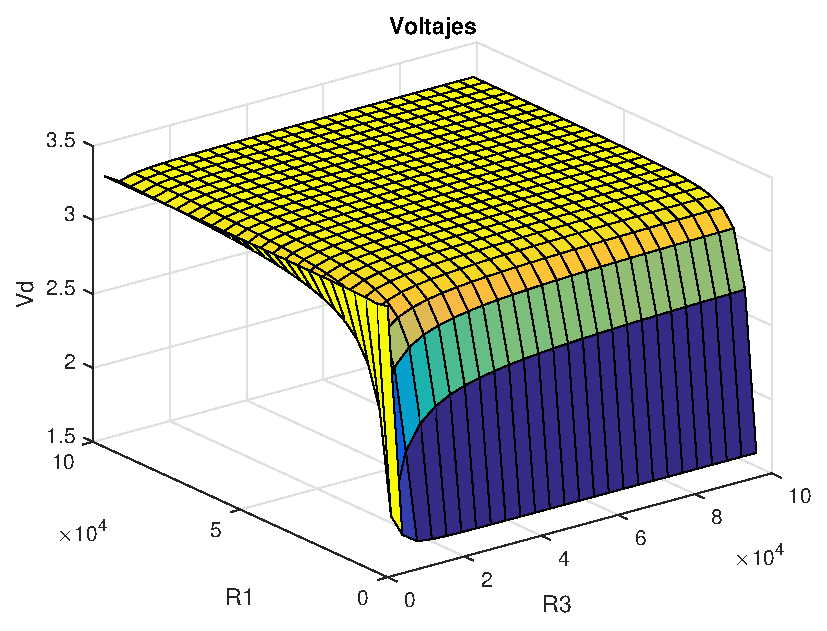
\includegraphics[width=0.6\linewidth]{MATLAB/ej2Vd.eps}
        \caption{f=1kHz}
        \label{fig:ej2Vd}
    \end{center}
\end{figure}

\begin{figure}[ht]
    \begin{center}
        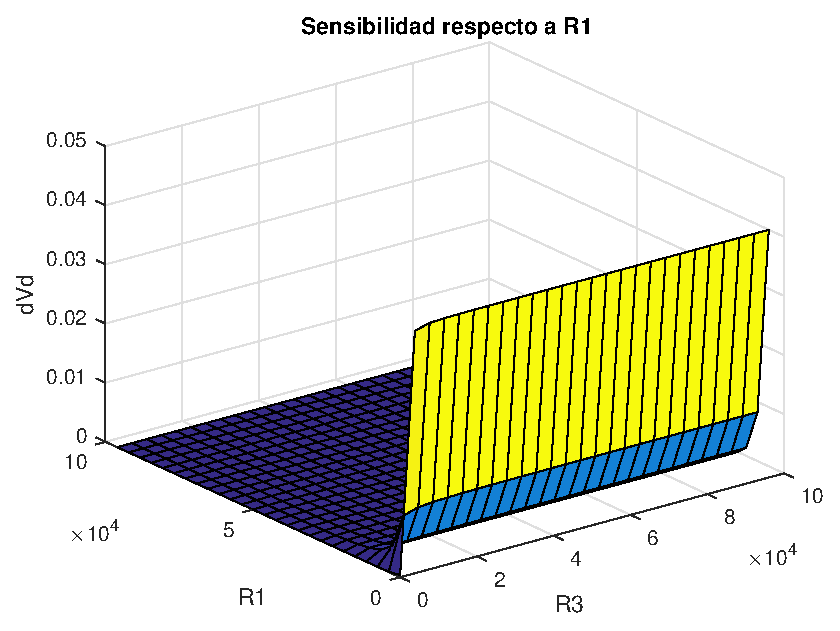
\includegraphics[width=0.45\linewidth]{MATLAB/ej2dVd1.eps}
        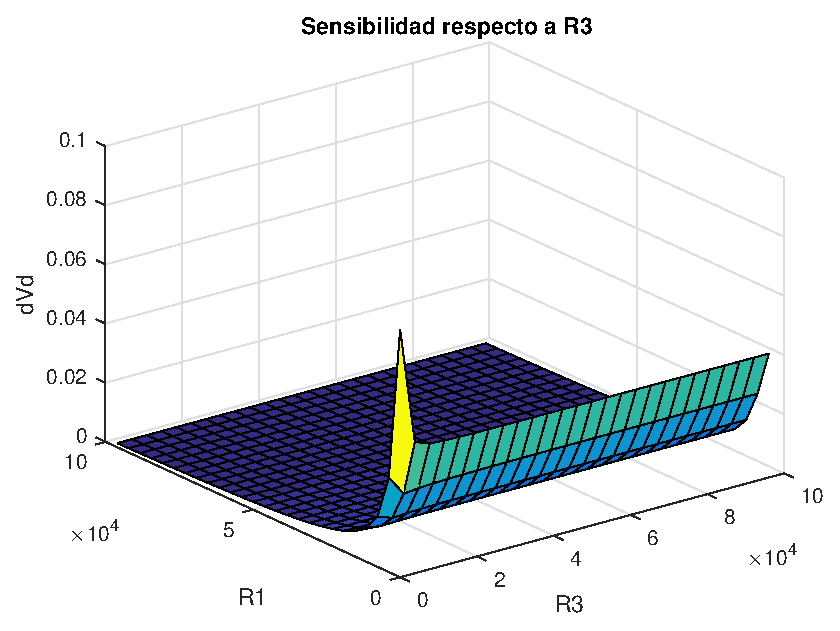
\includegraphics[width=0.45\linewidth]{MATLAB/ej2dVd3.eps}
        \caption{Sensibilidades a f=1kHz}
        \label{fig:ej2dVd}
    \end{center}
\end{figure}

\section{Mediciones}
Con el puente diseñado realizamos las siguientes mediciones mediante el uso de osciloscopio
y multímetro.

\begin{table}[ht]
    \begin{center}
        \begin{tabular}{|c|c|c|c|c|}
            \toprule
            F Generador ($\si{\hertz}$)& $R_1 (\si{\ohm})$& $R_3 (\si{\ohm})$& F Calculada ($\si{\hertz}$)& Error $\%$ \\
            \midrule
            2300&673&674&2363.103&2.67\\
            2000&796&799&1995.677&0.217\\
            1700&935&949&1679.590&0.616\\
            1400&1142&1136&1397.327&0.191\\
            1100&1466&1440&1095.398&0.420\\
            800&1990&1887&821.311&2.595\\
            500&3188&3160&501.438&0.287\\
            200&7996&7971&199.355&0.323\\
            \bottomrule
        \end{tabular}
    \end{center}
\end{table}

\section{Errores}
El error relativo al realizar las mediciones fue de aproximadamente $1 \% $. No hay un 
patrón específico en cuanto el error, ya que principalmente se debe a la sensibilidad del 
osciloscopio al medir ruido. Para considerar que el puente llegaba al equilibrio consideramos 
como aproximadamente 0 a valores menores a $3\si{\milli\volt}pp$ medidos con el multímetro y valores menores a 
$125\si{\milli\volt}pp$ medidos con el osciloscopio.

El rango de medición es mayor al requerido ya que para poder implementar el puente utilizamos 
resistencias de valores nominales disponibles en el laboratorio. El rango de variación de las 
resistencias fue entonces $\sim (680 \si{\ohm}; 1180 \si{\ohm})$. Otro factor de error fue que
para los cálculos tomamos los valores nominales de los capacitores, pero eran levemente 
menores y además su capacidad varía con la frecuencia.


\section{Conclusión}

Luego de realizar los cálculos de sensibilidades y realizar mediciones con el puente se concluye que es posible medir con el mismo frecuencias en el rango de 200 a  2000 Hz con buena precisión. Además el hecho de que el puente tenga un solo valor de R que haga que lo equilibre para cada frecuencia, permite una calibración y medición relativamente sencilla de las frecuencias deseadas.